\pdfoutput=1
\documentclass[10pt]{beamer}

%STANDARD PREAMBLE
%https://tex.stackexchange.com/questions/68821/is-it-possible-to-create-a-latex-preamble-header
\usepackage{../../rsrc/beamer_preamble}

%% ALLOW FOR ITEMIZE ENVIRONMENTS WITH NO PRECEDING
% SPACING, IF DESIRED
% Reference: https://tex.stackexchange.com/questions/86054/how-to-remove-the-whitespace-before-itemize-enumerate
%\usepackage{enumitem}% http://ctan.org/pkg/enumitem 
\usepackage{paralist}

% RANDOM VARIABLE
\newcommand{\x}{X}
\newcommand{\y}{Y}

%SUMS
\newcommand{\sumn}{\sum_{i=1}^{n}}


% ASSIGNMENTS
\newcommand{\assign}{z} %hardassignments
\newcommand{\Assign}{Z}
\newcommand{\soft}{r} %soft assignments

%%%% SUPPORT MAKING \subsectionpage
\AtBeginSection{\frame{\sectionpage}}
\AtBeginSubsection{\frame{\subsectionpage}}

\title{Hidden Markov Models}

\begin{document}

\maketitle


\begin{frame}{Acknowledgements}
An important resource for these slides was Christopher Bishop's \textit{Pattern Recognition and Machine Learning}.
\end{frame}

\begin{frame}{Hidden Markov Models}
\begin{sblock}{The model}
\begin{minipage}{0.6\textwidth}
\begin{itemize}
\item Observations $x_1, ..., x_n$.
\item  Latent variables $\mathbf{z}_n$ encode class (1-of-K encoding scheme).Assume a data point belongs to exactly one group or class out of K possibilities,
\item  Parameters $\theta = \{ A, \pi, \phi\}$
\begin{itemize} 
\item Transition probabilities $p(\mathbf{z}_n | \mathbf{z}_{n-1})$ given by $\mathbf{A}$, where $A_{jk} = p(z_{nk} = 1 | z_{n-1, j}= 1 )$
\item Emission probabilities $p(\mathbf{x}_n | \mathbf{z_n}, \phi)$ governed by $\phi$. (E.g. $\phi = \{\mu_k, \Sigma_k\}_{k=1}^K$)
\item Distribution of $\mathbf{z}$ given by $\pi$: $\pi_k = p(z_{1k}=1)$
\end{itemize}
\end{itemize}
\end{minipage} 
\hfill
\begin{minipage}{0.3\textwidth}
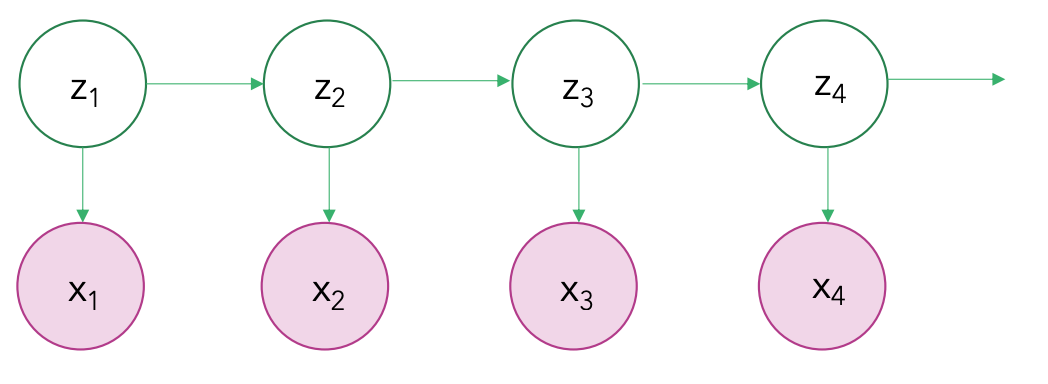
\includegraphics[width=\textwidth]{images/hmm}
\end{minipage} 

\end{sblock}
\end{frame}

\begin{frame}{Hidden Markov Models}

\begin{minipage}{0.5\textwidth}
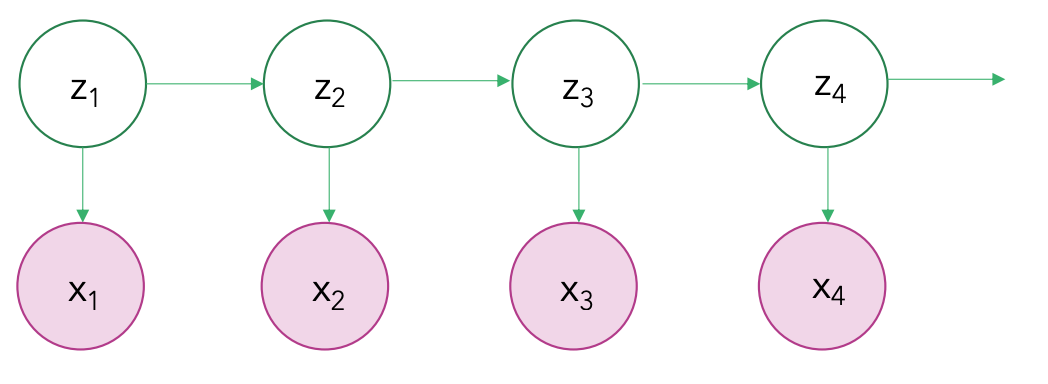
\includegraphics[width=\textwidth]{images/hmm}
\end{minipage} 

\vfill
\begin{minipage}{0.5\textwidth}
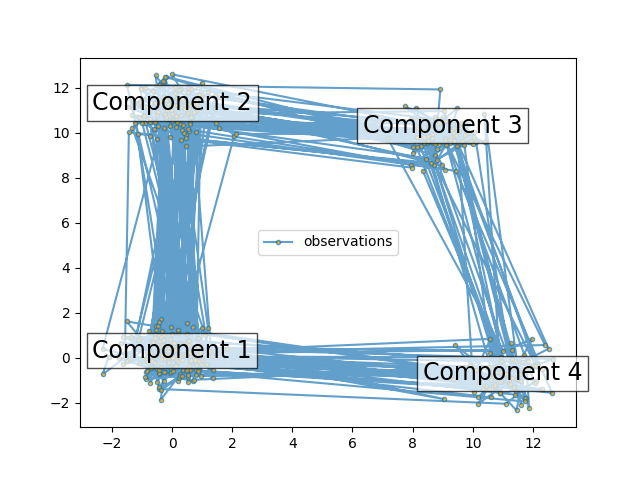
\includegraphics[width=\textwidth]{images/hmm-sampling}
\end{minipage} 

\end{frame}

\begin{frame}{Hidden Markov Models}
\begin{sblock}{Likelihood}
$$P(X| \theta) = \sum_{Z} P(X, Z | \theta)$$
\end{sblock}

\begin{sblock}{What would be hard about maximizing the likelihood?}

\end{sblock}

\end{frame}

\begin{frame}{Hidden Markov Models}
\begin{sblock}{Likelihood}
$$P(X| \theta) = \sum_{Z} P(X, Z | \theta)$$
\end{sblock}

\begin{sblock}{What would be hard about maximizing the likelihood?}
\begin{itemize}
\item No closed-form solution for maximum likelihood
\item The number of terms in the summation goes as $K^N$
\end{itemize}
\end{sblock}

%\begin{sblock}{Clustering and classification}
%Clustering is the ``unsupervised" counterpart to classification.   There is no training data and no labels, only one, unlabeled data set. 
%\end{sblock}

\end{frame}

\begin{frame}
\begin{sblock}{Complete data likelihood}
$$p(X, Z | \theta) = p(\mathbf{z}_1| \pi) \prod_{n=2}^N p(\mathbf{z}_n | \mathbf{z}_{n-1}, A) \prod_{m=1}^N p(\mathbf{x}_m | \mathbf{z}_m, \phi)$$
\end{sblock} 
\begin{sblock}{EM}
E : Compute $$Q(\theta, \theta^{(old)}) = \mathbb{E}_{Z | X, \theta^{(old)}} \ln p(X, Z | \theta).$$
M : Find $\theta$ to maximize $Q(\theta, \theta^{(old)})$.
\end{sblock}
\end{frame}

\begin{frame}
\begin{equation*}
\begin{split}
p(X, Z | \theta) &= p(\mathbf{z}_1| \pi) \prod_{n=2}^N p(\mathbf{z}_n | \mathbf{z}_{n-1}, A) \prod_{m=1}^N p(\mathbf{x}_m | \mathbf{z}_m, \phi) \\
&=(\prod_{k=1}^{K} \pi_k^{z_{1k} )}(\prod_{n=1}^N\prod_{k=1}^K \prod_{j=1}^K A_{jk}^{z_{n-1,j}z_{nk} })( \prod_{m=1}^N \prod_{k=1}^K z_{mk} p(\mathbf{x}_n | \phi_k)
 \end{split}
 \end{equation*}
%$$\implies \ln p (X, Z | \theta)$$
\begin{sblock}{E-step}
Define: $\gamma(\mathbf{z}_n)  = p(\mathbf{z}_n | \mathbf{X}, \theta^{(old)})$ Note: $\gamma(z_{nk}) = \mathbb{E}[z_{nk}] $ \\%= \sum_{\mathbf{z_n}} \gamma(\mathbf{z}) z_{nk}$\\
$\xi( \mathbf{z}_{n-1}, \mathbf{z}_n) = p(\mathbf{z}_{n-1}, \mathbf{z}_n |  \mathbf{X}, \theta^{(old)}).$ Note: $\xi(z_{n-1, j}, z_{nk} ) = \mathbb{E}[z_{n-1,j}z_{nk}] $\\%= \sum  \gamma(\mathbf{z}) z_{n-1, j} z_{nk} $ \\
Evaluate $\gamma, \xi$ (how? forward backward algorithm). Then can compute:
%$$\ln p(X,Z | \theta) = $$
\begin{equation*}
\begin{split}
Q(\theta, \theta^{(old)}) =& \mathbb{E}_{Z | X, \theta^{(old)}} \ln p(X, Z | \theta) \\
&= \sum_{k=1}^K \gamma(z_{1k}) \ln \pi_k + \sum_{n=2}^N \sum_{j=1}^K \sum_{k=1}^K \xi(z_{n-1, j} z_{nk}) \ln A_{jk}\\
&+ \sum_{n=1}^N\sum_{k=1}^K \gamma(z_{nk}) \ln p(\mathbf{x}_n | \phi_k)
\end{split}
\end{equation*}
%%M: Find $\theta$ to maximize $Q(\theta, \theta^{(old)})$.
\end{sblock}
\end{frame}


\begin{frame}
\begin{equation*}
\begin{split}
Q(\theta, \theta^{(old)}) =& \mathbb{E}_{Z | X, \theta^{(old)}} \ln p(X, Z | \theta) \\
&= \sum_{k=1}^K \gamma(z_{1k}) \ln \pi_k + \sum_{n=2}^N \sum_{j=1}^K \sum_{k=1}^K \xi(z_{n-1, j} z_{nk}) \ln A_{jk}\\
&+ \sum_{n=1}^N\sum_{k=1}^K \gamma(z_{nk}) \ln p(\mathbf{x}_n | \phi_k)
\end{split}
\end{equation*}
\begin{sblock}{M-step: Find $\theta$ to maximize $Q(\theta, \theta^{(old)})$.}
$\pi_k = \frac{\gamma(z_{1k})}{\sum_{k=1}^K \gamma(z_{1k})}$, $A_{jk} = \frac {\sum_{n=2}^N \xi(z_{n-1, j} z_{nk})}{\sum_{l=1}^K\sum_{n=2}^N \xi(z_{n-1,j},z_{nl})}$ \\
Result of maximization with respect to $\phi$ depends on choice of emission probabilities.
\end{sblock}
\end{frame}

\begin{frame}
\begin{sblock}{M-step: Find $\theta$ to maximize $Q(\theta, \theta^{(old)})$.}
$$\pi_k = \frac{\gamma(z_{1k})}{\sum_{k=1}^K \gamma(z_{1k})}, A_{jk} = \frac {\sum_{n=2}^N \xi(z_{n-1, j} z_{nk})}{\sum_{l=1}^K\sum_{n=2}^N \xi(z_{n-1,j},z_{nl})}$$ \\
Result of maximization with respect to $\phi$ depends on choice of emission probabilities.\\
E.g if $p(\mathbf{x}| \phi_k) = \text{Normal}(\mathbf{x}|\mu_k, \Sigma_k)$\\
$$\mu_k = \frac{\sum_{n=1}^N \gamma(z_{nk})\mathbf{x}_n}{\sum_{n=1}^N \gamma(z_{nk})}, \Sigma_k = \frac{\sum_{n=1}^N \gamma(z_{nk})(\mathbf{x}_n - \mu_k)(\mathbf{x}_n - \mu_k)^T}{\sum_{n=1}^N \gamma(z_{nk})}$$
\end{sblock}
\begin{sblock}{EM for HMMs summary:}
Alternate between updating $\gamma, \xi$ and updating $\pi, A, \phi$.
\end{sblock}
\end{frame}

\begin{frame}
\begin{sblock}{How to efficiently calculate $\gamma, \xi$ for the E-step?}
Use a two-stage message passing algorithm, the \textit{forward-backward algorithm} to compute.\\
For details and derivation, see, e.g. Christopher Bishop's \textit{Pattern Recognition and Machine Learning} sec. 13.2.2. 
\end{sblock}
\end{frame}



%\begin{frame}{Example: Image Segmentation}
%\scriptsize
%\begin{sblock}{Image Segmentation}
%\bf{Image segmentation} is the problem of partitioning an image into ``coherent" regions.  The problem is not well-posed: Its solution depends on the meaning of ``coherent".
%\end{sblock}
%
%\begin{sblock}{Example}
%\includegraphics[width=\textwidth]{images/image_segmentation}
%\end{sblock}
%
%\begin{sblock}{Segmentation as a clustering problem}
%\begin{itemize}
%\item For each pixel, place a small window around the pixel.  Extract features (measurements) from this window.  For the $i$-th pixel, represent measurements by a vector $x_i$.
%\item Compute a clustering of the data $x_1, ..., x_n$ with K clusters.
%\item Each cluster represents one segment.  In the images above, one cluster is colored blue, one green, one red.
%\end{itemize}
%
%\end{sblock}

%\end{frame}
\end{document}
